\documentclass[aspectratio=169, 12pt]{beamer}

% ── Theme ─────────────────────────────────────────────────────────────────────
\usetheme{Madrid}
\usecolortheme{seahorse}
\setbeamertemplate{navigation symbols}{}
\setbeamertemplate{footline}[frame number]

% ── Packages ──────────────────────────────────────────────────────────────────
\usepackage{amsmath, amssymb}
\usepackage{graphicx}
\usepackage{booktabs}
\usepackage{xcolor}
\usepackage{tikz}
\graphicspath{{../../plots/}}   % pull figures from ../plots/

% ── Custom colors (match Python palette) ──────────────────────────────────────
\definecolor{trivial}{HTML}{d62728}
\definecolor{critical}{HTML}{2ca02c}
\definecolor{topological}{HTML}{1f77b4}
\definecolor{edgemode}{HTML}{e377c2}

% ── Macros ────────────────────────────────────────────────────────────────────
\newcommand{\cdag}{c^{\dagger}}
\newcommand{\gA}{\gamma_{A,j}}
\newcommand{\gB}{\gamma_{B,j}}
\newcommand{\winding}{\nu}

% ── Title ─────────────────────────────────────────────────────────────────────
\title[Kitaev Chain — Block 1]{Majorana Modes in the Machine}
\subtitle{Block 1: The Physics Bridge}
\author{Dobromir Stoev\\ Edgar Harutyunyan\\ Guilherme Schewtschik\\ Jaskaran Singh\\ Zhengyi Liu\\ Zhenming Shi}
\institute{Advanced Seminar — AI-Augmented Theoretical Physics}
\date{\today}

% ══════════════════════════════════════════════════════════════════════════════
\begin{document}

\begin{frame}
  \titlepage
\end{frame}

% ── Outline ───────────────────────────────────────────────────────────────────
\begin{frame}{Outline}
  \tableofcontents
\end{frame}

% ══════════════════════════════════════════════════════════════════════════════
\section{The Kitaev Hamiltonian \& Edge Modes}

\begin{frame}{Starting point: the lattice Kitaev Hamiltonian}
  \begin{equation}
    H_K = -\mu \sum_j \cdag_j c_j
          - t \sum_j \!\bigl(\cdag_j c_{j+1} + \mathrm{h.c.}\bigr)
          + \Delta \sum_j \!\bigl(\cdag_j \cdag_{j+1} + \mathrm{h.c.}\bigr)
  \end{equation}
  \begin{columns}[T]
    \begin{column}{0.45\textwidth}
      \textbf{Physical ingredients}
      \begin{itemize}
        \item Spinless (or spin-polarized) fermions
        \item Nearest-neighbor hopping $t$
        \item $p$-wave pairing $\Delta \in \mathbb{R}$
        \item Chemical potential $\mu$ tunes filling
      \end{itemize}
    \end{column}
    \begin{column}{0.45\textwidth}
    \centering
    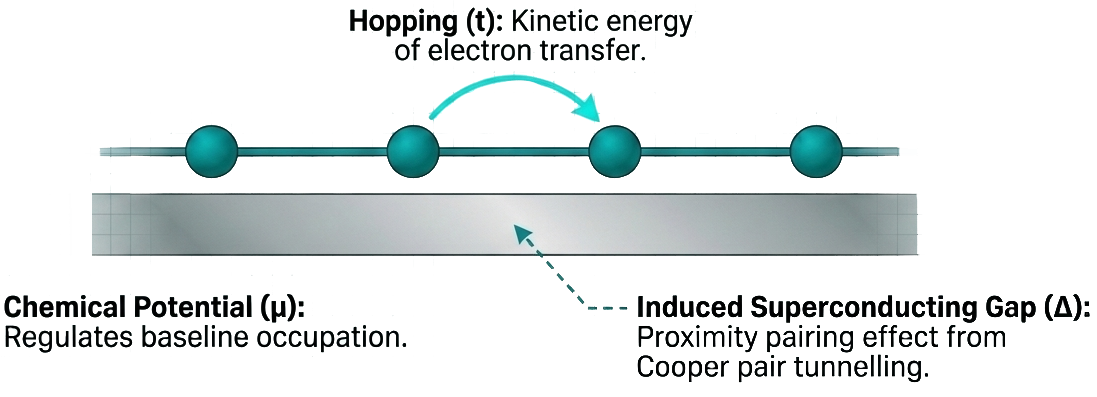
\includegraphics[width=\linewidth]{../../img/setup.png}
      
      \textbf{Questions we will answer}
      \begin{itemize}
        \item When does topology emerge?
        \item How do edge zero modes appear?
      \end{itemize}
    \end{column}
  \end{columns}
\end{frame}

\begin{frame}{Majorana Representation \& The ``Sweet Spot''}
  Ordinary fermions can be split into two Hermitian \textbf{Majorana operators}:
  \begin{equation}
    \gamma_{A,j} = \frac{c_j + \cdag_j}{\sqrt{2}}, \qquad
    \gamma_{B,j} = \frac{i(\cdag_j - c_j)}{\sqrt{2}}
  \end{equation}
  
  By rewriting $H_K$ in terms of Majoranas (see Appendix for details), we find a special limit:

  \begin{alertblock}{Sweet spot: $\mu = 0$, $t = \Delta$}
    The intra-site coupling vanishes. Only inter-site coupling $i\gamma_{B,j}\gamma_{A,j+1}$ survives.
    In a chain with open boundaries, this leaves \textbf{one unpaired Majorana zero-mode at each end}.
  \end{alertblock}

  \begin{block}{Why is this interesting?}
    These edge Majorana modes are \textbf{robust} (protected by topology) and candidates for \textbf{fault-tolerant quantum computation}.
  \end{block}
\end{frame}

% ── BdG Spectrum (Main Results) ───────────────────────────────────────────────
\section{Bulk Spectrum \& Phase Transition}

\begin{frame}{Bulk dispersion: topological / critical / trivial}
  Applying a Fourier transform and using the BdG formalism (see Appendix), the energy spectrum is given by:
  \begin{equation}
    E_k = \pm\sqrt{n_z(k)^2 + n_y(k)^2} = \pm\sqrt{(-\mu - 2t\cos k)^2 + (-2\Delta\sin k)^2}
  \end{equation}
  
  The topological phase transition occurs when the \textbf{bulk gap closes} ($E_k = 0$). This happens at $k=\{0, \pi\}$ when $\mu = \pm 2t$.

  \begin{center}
    \includegraphics[width=\linewidth]{block1_01_bulk_dispersion.png}
  \end{center}
\end{frame}

% ── Winding number ────────────────────────────────────────────────────────────
\section{Topological Invariant}

\begin{frame}{Winding number $\nu$}
  As $k$ sweeps the BZ, the vector $\mathbf{n}(k)=(n_z,n_y)$ traces a closed loop.
  \begin{equation}
    \theta_k = \arg(n_z + i n_y), \qquad
    \winding = \frac{1}{2\pi}\int_\mathrm{BZ} \partial_k\theta_k\, dk
  \end{equation}

  \begin{center}
    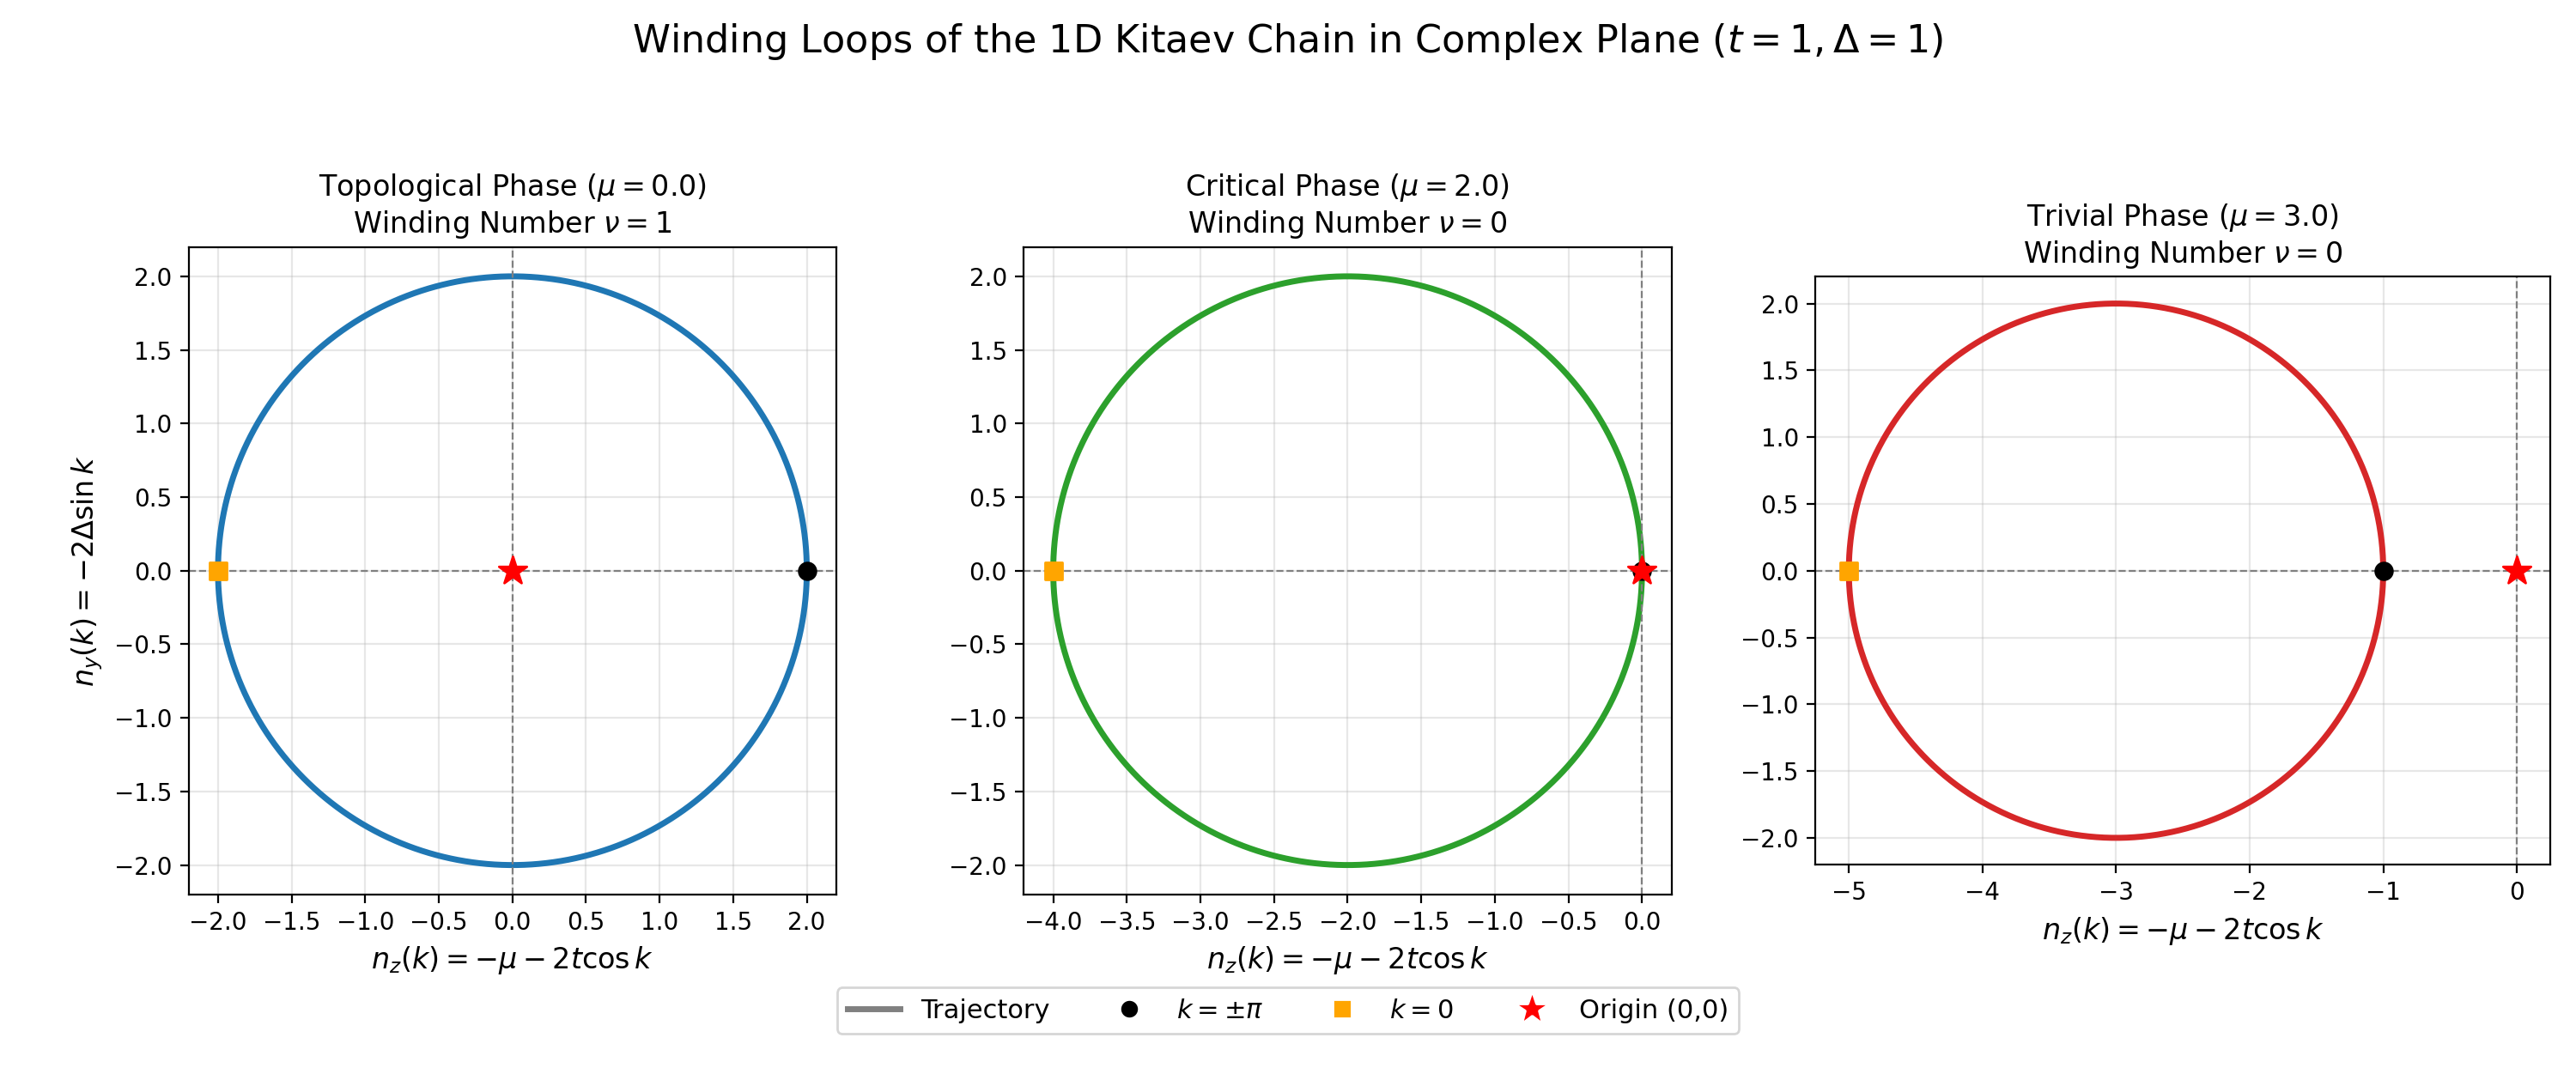
\includegraphics[width=0.6\linewidth]{block1_02_winding_loops.png}
  \end{center}
  \begin{itemize}
    \item $\nu=0$: loop does \emph{not} enclose origin $\to$ trivial
    \item $|\nu|=1$: loop winds once around origin $\to$ topological
  \end{itemize}
\end{frame}

\begin{frame}{Phase diagram}
  \begin{center}
    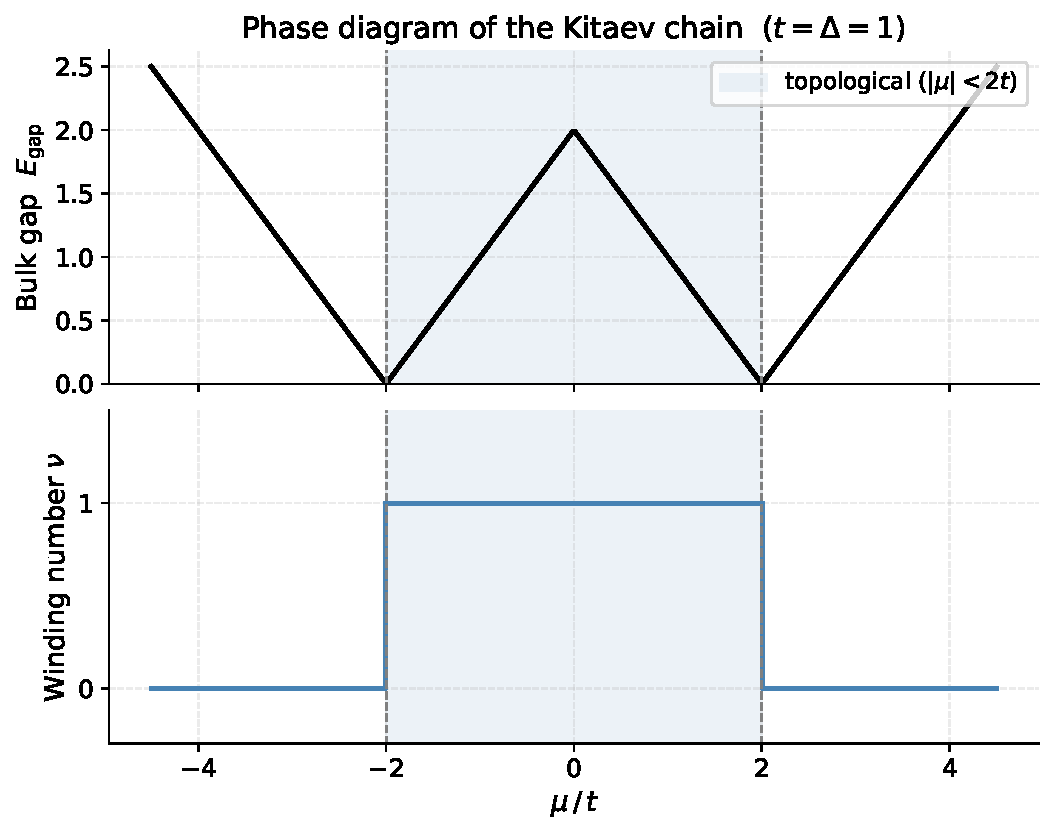
\includegraphics[width=0.5\linewidth]{block1_03_phase_diagram.pdf}
  \end{center}
  Bulk gap vanishes at $\mu = \pm 2t$; winding number jumps across the transition.
\end{frame}


% ── Topology Conceptual Bridge ────────────────────────────────────────────────
\section{Topology \& Protection}

\begin{frame}{Topology: Continuity and Invariance}
      \begin{itemize}
        \item \textbf{Topological Equivalence}: Two shapes are equivalent if they can be transformed into each other via ``continuous deformation'' (stretching, bending).
      \end{itemize}
  \begin{itemize}
    \item \textbf{Invariants}: Properties that remain unchanged during deformation (e.g., number of holes / Genus).
    \item \textbf{Physical Link}: Tuning Hamiltonian parameters ($t, \mu$) is essentially a ``continuous deformation'' of the wave function.
  \end{itemize}
  \begin{block}{Core Intuition}
    You cannot turn a {\color{trivial}Sphere} (0 holes) into a {\color{topological}Donut} (1 hole) without ``tearing'' the surface (Gap Closing).
  \end{block}
\end{frame}

\begin{frame}{Topological invariant: The Winding Number}
  \begin{columns}
    \begin{column}{0.45\textwidth}
      \begin{figure}
        \centering
        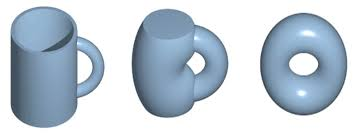
\includegraphics[width=1.1\textwidth]{../../img/donuts.png}
      \end{figure}
      with Genus 1
    \end{column}
    \begin{column}{0.45\textwidth}
      \begin{figure}
        \centering
        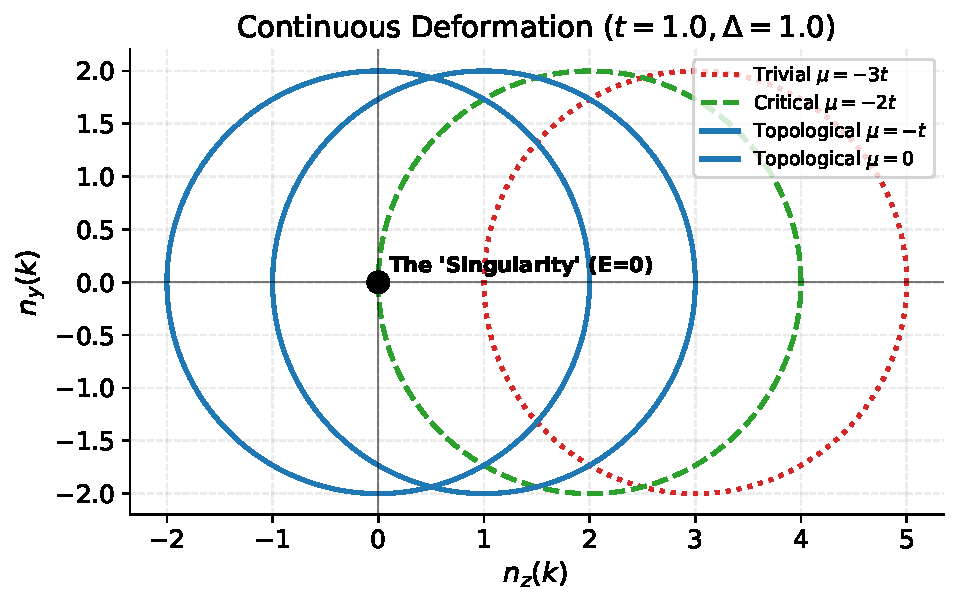
\includegraphics[width=0.9\textwidth]{block1_02_trajectory_deformation.pdf}
      \end{figure}
      winding number $\nu = 1$
    \end{column}
  \end{columns}
  \begin{alertblock}{What is Protection?}
    As long as the circle doesn't cross the origin (Gap remains open), parameter fluctuations only ``deform'' the circle but cannot change the \textbf{integer} winding number.
  \end{alertblock}
\end{frame}

% ── Summary ───────────────────────────────────────────────────────────────────
\section{Summary}

\begin{frame}{Block 1 — key takeaways}
  \begin{enumerate}
    \item The Kitaev Hamiltonian hosts \textbf{two phases} separated by gap closings at $\mu=\pm 2t$.
    \item Majorana representation reveals the \textbf{sweet-spot} picture directly ($\mu=0,\,t=\Delta$).
    \item The BdG d-vector winding number $\nu\in\{0,1\}$ is the \textbf{topological invariant}.
  \end{enumerate}
  \vfill
  \textbf{Next (Block 2):} Finite size \& edge modes → Jordan–Wigner transform → qubit encoding → quantum circuit for ground-state preparation.
\end{frame}


% ══════════════════════════════════════════════════════════════════════════════
% ── Appendix ──────────────────────────────────────────────────────────────────
\appendix

\begin{frame}
  \centering
  \Huge \textbf{Appendix}
\end{frame}

\begin{frame}{Appendix A: Full Majorana Representation}
  Recall the Majorana operators:
  \begin{equation}
    \gamma_{A,j} = \frac{c_j + \cdag_j}{\sqrt{2}}, \qquad
    \gamma_{B,j} = \frac{i(\cdag_j - c_j)}{\sqrt{2}}
  \end{equation}
  where $\{\gamma_{\alpha,i}, \gamma_{\beta,j}\} = 2\delta_{\alpha\beta}\delta_{ij}$.

  \medskip
  Rewriting the full Kitaev Hamiltonian in the Majorana basis yields:
  \begin{equation}
    H_K = -\mu\!\sum_j \!\Bigl(i\gA\gB + \tfrac{1}{2}\Bigr)
          + i\!\sum_j \!\Bigl[
              (\Delta+t)\,\gamma_{B,j}\gamma_{A,j+1}
             +(\Delta-t)\,\gamma_{A,j}\gamma_{B,j+1}
            \Bigr]
  \end{equation}
  \emph{Note how setting $\mu=0$ and $t=\Delta$ simplifies this to just the $i\gamma_{B,j}\gamma_{A,j+1}$ term.}
\end{frame}

\begin{frame}{Appendix B: Momentum Space Mapping}
  The tight-binding Hamiltonian in real space:
  \begin{equation}
    H = \sum_{j} \left[ -t(c^\dagger_j c_{j+1} + \text{h.c.}) - \mu\left(c^\dagger_j c_j - \frac{1}{2}\right) + \Delta(c_j c_{j+1} + c^\dagger_{j+1} c^\dagger_j) \right]
  \end{equation}
  Applying the Fourier transform $c_j = \frac{1}{\sqrt{N}} \sum_{k} e^{ikj} c_k$, the kinetic and chemical potential terms diagonalize trivially. The pairing term requires antisymmetrization due to fermionic statistics ($c_k c_{-k} = -c_{-k} c_k$):
  \begin{equation}
    \Delta \sum_k e^{ik} c_k c_{-k} = \Delta \sum_{k>0} (e^{ik} - e^{-ik}) c_k c_{-k} = 2i\Delta \sum_{k>0} \sin(k) c_k c_{-k}
  \end{equation}
  This isolates the odd-parity $p$-wave superconducting nature of the model in momentum space.
\end{frame}

\begin{frame}{Appendix C: BdG Formalism and Pseudospin}
  Use the Nambu spinor $\Psi_k = \begin{pmatrix} c_k \\ c^\dagger_{-k} \end{pmatrix}$ to cast $H$ into a bilinear form:
  \begin{equation}
    H = \sum_{k>0} \Psi^\dagger_k h(k) \Psi_k, \quad
    h(k) = \begin{pmatrix} \xi_k & 2i\Delta\sin(k) \\ -2i\Delta\sin(k) & -\xi_k \end{pmatrix}
  \end{equation}
  where the normal-state dispersion is $\xi_k = -\mu - 2t\cos(k)$. 
  
  Expanding $h(k)$ in Pauli matrices:
  \begin{equation}
    h(k) = n_y(k)\sigma^y + n_z(k)\sigma^z \implies 
    \begin{cases}
      n_z(k) = -\mu - 2t\cos(k) \\
      n_y(k) = -2\Delta\sin(k)
    \end{cases}
  \end{equation}
  Diagonalizing this yields the bulk dispersion $E_k = \pm\sqrt{n_z(k)^2 + n_y(k)^2}$.
\end{frame}

\end{document}